\documentclass[kravspec.tex]{subfiles}
\begin{document}
\section{Generel beskrivelse}
Dette afsnit i kravspecifikationen vil give et overodnet billede af de krav der er blevet opstillet for udviklingen af systemet.
	
\subsection{Systembeskrivelse}
\begin{figure}[h]
\centering
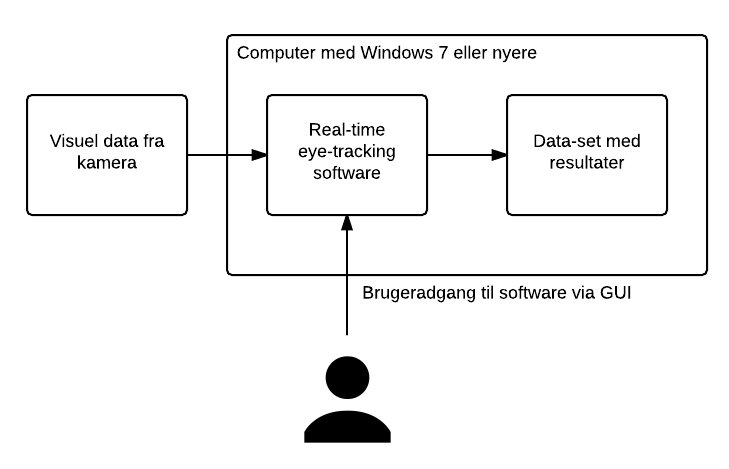
\includegraphics[width=0.7\linewidth]{../Systemdiagram.png}
\caption[Systemdiagram]{Systemdiagram for Real-time eye-tracking}
\label{fig:Systemdiagram}
\end{figure}
Der ønskes udviklet et system som kan indsamle videodata fra et kamera og derefter anvende dataen til
at bestemme hvor en forsøgsperson kigger hen på en specifik skærm. Systemet skal derudover videregive
denne information til brugeren via koordinater samt en graf der repræsenterer den skærm forsøgspersonen
ser på.
\\
\indent
Før dataopsamling skal en indledende kalibrering af systemet gennemføres. Dette gøres ved at et gitter med
specifikke punkter indlæses på forsøgspersonsskærmen. Derefter bedes forsøgspersonen se på specifikke punkter
på skærmen, og sammenhængen imellem de målte punkter og de kendte punkter kan anvendes til at finde en
homografisk mapning. Efter denne kalibrering kan systemet anvendes.
\\
\indent
Systemet udvikles med henblik på en standard anvendelsesmåde, med mulighed for brugerdefinerede anvendelses-
måder. Standardanvendelsen omhandler at vælge en sti og et filnavn, hvorefter dataopsamling umiddelbart begynder.
Under dataopsamlingen vil gazevectoren løbende blive præsenteret for brugeren på brugerskærmen. Når brugeren er 
færdig kan opsamlingen stoppes, og dataopsamlingen gemmes i den tidligere valgte fil. Bemærk at den algoritme
der anvendes til behandling af data her er forudbestemt.
\\
(Hvis brugeren ønsker at bruge en anden algoritme kan denne indlæses. Den kan også indskrives direkte i
GUI'en, og derefter gemmes. Formålet med dette er at kunne indrette systemet efter specifikke behov, og
hurtigt indhente de opsætninger til fremtidig brug. Eventuelt kan andre variabler indtastes ved systemstart) 
\\
\indent
I de følgende afsnit fremgår det hvorledes det udviklede system indgår i det samlede system.


\subsection{Aktører}
\begin{figure}[h]
\centering
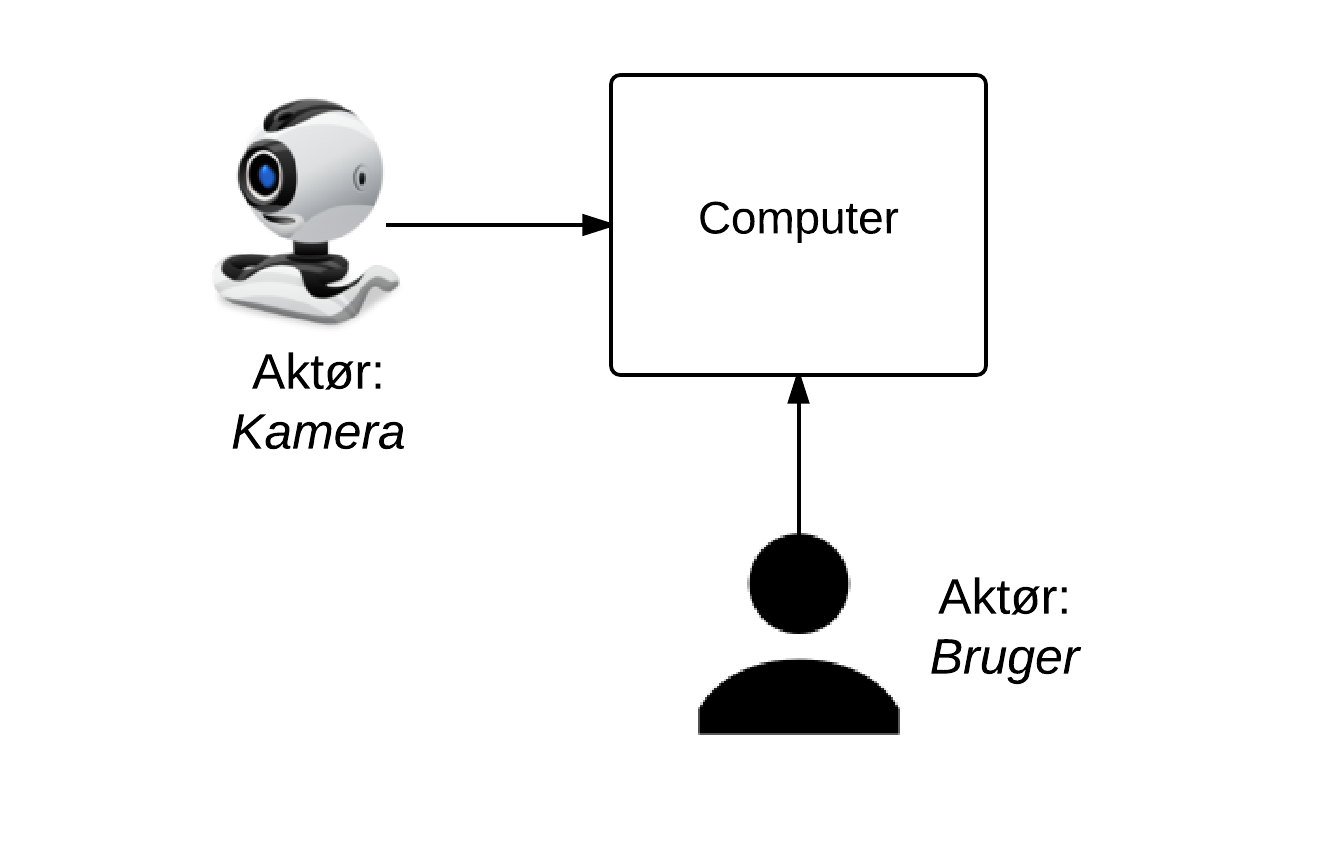
\includegraphics[width=0.7\linewidth]{../Actors}
\caption{Systemets aktører}
\label{fig:Actors}
\end{figure}

En række af de kommende funktionelle krav vil blive opstillet som use-cases. Følgende er beskrivelser for de enkelte aktører: \\
\\
\begin{tabular}{| l | p{10cm} |}
	\hline 
	\textbf{Navn} & \textit{Bruger} \\ \hline
	\textbf{Beskrivelse} & Brugeren er personen der tilgår systemet via et grafisk user interface.\\ \hline
\end{tabular}
\newline
\vspace*{0.7 cm}
\newline
\begin{tabular}{| l | p{10cm} |}
	\hline 
	\textbf{Navn} & \textit{Kamera} \\ \hline
	\textbf{Beskrivelse} & Systemet vil snakke sammen med et kamera, hvis formål er at levere visuelt data.\\ \hline
\end{tabular}

\subsection{Systemets begrænsninger}
\begin{enumerate}
	\item Systemet kan ikke forventes at køre realtime (100 fps) udenfor standard anvendelse.
\item 
Systemet kan ikke håndtere briller på forsøgspersonen.
\item 
Systemet kan ikke anvendes uden indledende kalibrering.
\item 
Systemet kan ikke håndtere hovedbevægelser uden for X / X / X.
\end{enumerate}
\end{document}